\chapter{Benutzerverwaltung}
\label{Benutzerverwaltung}
In einem ASP.NET MVC Projekt ist bereits eine vollst�ndige Benutzerverwaltung integriert,
die wir auch in unserem Projekt benutzen wollen. Durch die integrierte Benutzerverwaltung 
sind Webseiten zur Registrierung und f�r den Login / Logout bereits fertig. 

\begin{figure}[H]
\centering
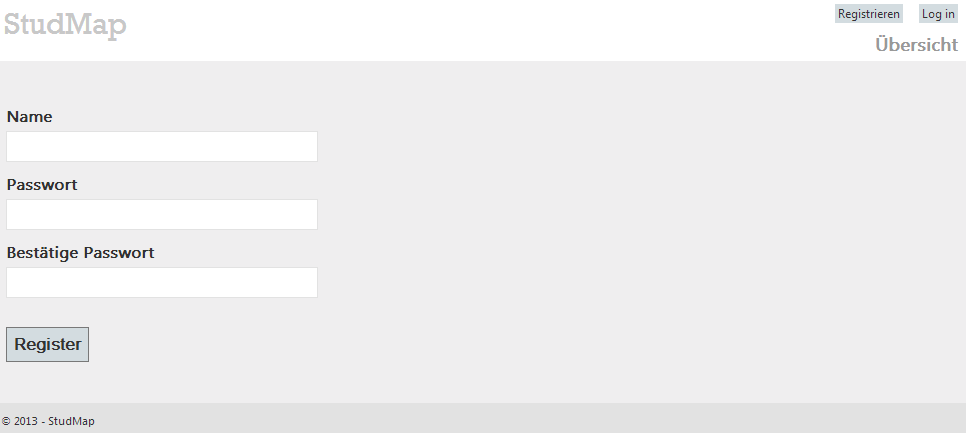
\includegraphics[width=0.7\linewidth]{../Bilder/RegisterSite}
\caption{Webseite zur Registrierung im StudMap Admin}
\label{fig:RegisterSite}
\end{figure}

F�r die Benutzerverwaltung verwendet das ASP.NET MVC Projekt folgende Datenbankstruktur:
\begin{figure}[H]
\centering
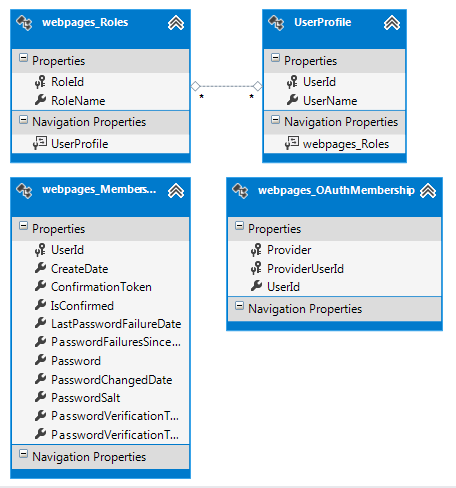
\includegraphics[scale=0.7]{../Bilder/GeneratedUserEntities}
\caption{Datenbankstruktur der integrierten Benutzerverwaltung}
\label{fig:GeneratedUserEntities}
\end{figure}

F�r unser Projekt sind nur die drei Tabellen \texttt{UserProfile}, \texttt{webpages\_Roles} und \texttt{webpages\_Membership} relevant. Wie im Domain Model bereits beschrieben unterscheiden wir zwischen den Benutzerrollen Benutzer und Administrator. Jeder Anwender kann sich in mehreren Benutzerrollen befinden. Zus�tzlich sind in der Tabelle \texttt{webpages\_membership} weitere Anwenderdaten wie beispielsweise das Datum der Registrierung das Passwort hinterlegt. Damit ist die Benutzerverwaltung f�r den Administrationsbereich vollst�ndig.

\begin{wrapfigure}{r}{0.4\textwidth}
\vspace{-40pt}
 \begin{center}
   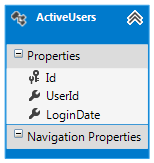
\includegraphics[scale=0.9]{../Bilder/ActiveUsersEntity}
 \end{center}
 \vspace{-30pt}
\end{wrapfigure}

Um die (beispielsweise �ber das Smartphone) am System angemeldeten Clients zu verwalten haben wir eine weitere Tabelle \texttt{ActiveUsers} hinzugef�gt.

F�r den StudMap Admin gen�gt die bereits integrierte Benutzerverwaltung. Allerdings ben�tigen wir noch eine Schnittstelle, damit auch die Web bzw. Smartphone Clients auf die Benutzerverwaltung zugreifen k�nnen.
Siehe dazu Kapitel \nameref{Verwendung_Benutzerschnittstelle}.
